\documentclass[aspectratio=169]{beamer}

\include{preamble}

\addbibresource{Presentation.bib}
\DeclareCiteCommand{\citejournal}{}{\printfield{journaltitle}}{}{}

\input{notation}

\DeclareMathOperator{\Tr}{Tr}

\title{Superconducting Phase Stiffness and Coherence Length From a Finite Momentum Pairing Constraint}
\author{Tjark Sievers}
\date{May 2025}
\institute[]{Master's Colloquium}

\usetheme{CCMT}

\begin{document}
	

{
\setbeamertemplate{footline}{\empty}
\begin{frame}
	\titlepage
\end{frame}
}
\addtocounter{framenumber}{-1}

\begin{frame}
	\frametitle{
		Flat Band Graphene Systems\footnote[frame]{Band structure \citeauthor{tormaSuperconductivitySuperfluidityQuantum2022},  \href{https://doi.org/10.1038/s42254-022-00466-y}{10.1038/s42254-022-00466-y} (\citejournal{tormaSuperconductivitySuperfluidityQuantum2022} \citeyear{tormaSuperconductivitySuperfluidityQuantum2022})}\footnote[frame]{\citeauthor{caoUnconventionalSuperconductivityMagicangle2018},  \href{https://doi.org/10.1038/nature26160}{10.1038/nature26160} (\citejournal{caoUnconventionalSuperconductivityMagicangle2018} \citeyear{caoUnconventionalSuperconductivityMagicangle2018})}
	}
	
		
	\begin{columns}
		\begin{column}{0.45\textwidth}
			\begin{center}
				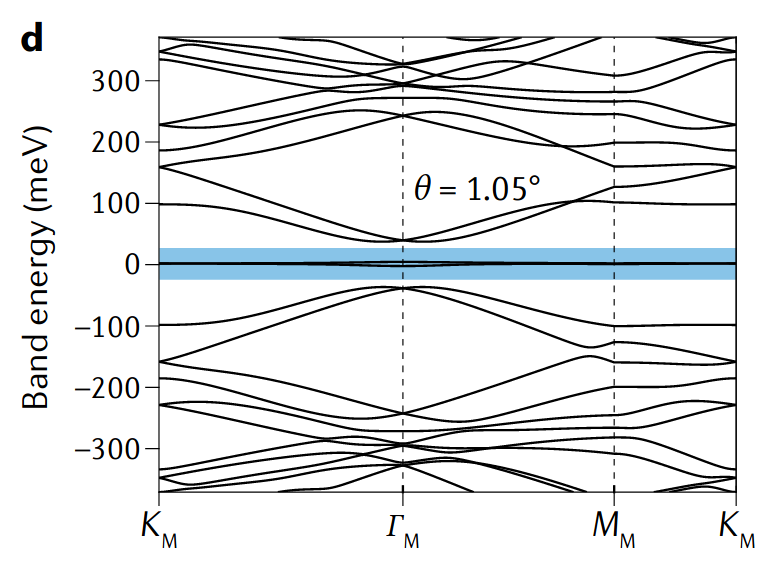
\includegraphics[width=\textwidth]{images/TBG band structure}
			\end{center}
		\end{column}
		\begin{column}{0.55\textwidth}
			\begin{center}
				
\includegraphics[width=0.8\textwidth]{images/TBG SC experiment}
			\end{center}
		\end{column}
	\end{columns}
\end{frame}

%\begin{frame}
%	\begin{columns}
%		\begin{column}{0.45\textwidth}
%			\begin{center}
%				
\includegraphics[width=\textwidth]{images/Uemura_plot}
%			\end{center}
%		\end{column}
%		\begin{column}{0.55\textwidth}
%			\begin{itemize}
%				\item TODO: mark graphene based systems
%				\item Uemura plot\footnote[frame]{Plot from \citeauthor{wittElectronCorrelationsUnconventional2024} \href{https://nbn-resolving.org/urn\%3Anbn\%3Ade\%3Agbv\%3A18-ediss-125247}{urn:nbn:de:gbv:18-ediss-125247} (\citeyear{wittElectronCorrelationsUnconventional2024}) with data from \citeauthor{nakagawaGatecontrolledBCSBECCrossover2021} \href{https://doi.org/10.1126/science.abb9860}{10.1126/science.abb9860} (\citeyear{nakagawaGatecontrolledBCSBECCrossover2021}), \citeauthor{uemuraDynamicSuperconductivityResponses2019} \href{https://doi.org/10.1103/PhysRevMaterials.3.104801}{10.1103/PhysRevMaterials.3.104801} (\citeyear{uemuraDynamicSuperconductivityResponses2019}), \citeauthor{pantaleonSuperconductivityCorrelatedPhases2023} \href{https://doi.org/10.1038/s42254-023-00575-2}{10.1038/s42254-023-00575-2} (\citeyear{pantaleonSuperconductivityCorrelatedPhases2023})}: \(T_{\mathrm{C}}\) compared to density of charge carriers (characterized by \(T_{\mathrm{F}}\))
%				\item 
%			\end{itemize}
%		\end{column}
%	\end{columns}
%\end{frame}

\begin{frame}
	\frametitle{Superconductivity in Flat-Band Systems}
	
	\begin{itemize}
		\item Superconductivity: pairing of electrons and phase coherence
%		\item Phase coherence is captured by superfluid phase stiffness \(D_{\mathrm{S}}\)
		\item Also enables superconducting current:
		\begin{equation}
			\vb{j} = D_{\mathrm{S}} \vb{A}
		\end{equation}
	\end{itemize}
	In single band:
	\begin{equation}
		D_{S, ij} \sim \sum_{\vb{k}} \pdv{\epsilon_{\vb{k}}}{k_i,k_j} \hspace{1cm} \text{Vanishes for a flat band!}
	\end{equation}
\end{frame}


\begin{frame}

	
	In multi-band systems\footnote{\citeauthor{peottaSuperfluidityTopologicallyNontrivial2015}, \href{https://doi.org/10.1038/ncomms9944}{10.1038/ncomms9944} (\citejournal{peottaSuperfluidityTopologicallyNontrivial2015} \citeyear{peottaSuperfluidityTopologicallyNontrivial2015})}:
	\begin{itemize}
		\item Conventional:
		\begin{equation}
			D_{\textrm{S}, 1, ij} \sim \sum_{\vb{k}} \pdv{\epsilon_{\vb{k}}}{k_i,k_j}
		\end{equation}
		\item Geometric: 
		\begin{equation}
			D_{\textrm{S}, 2, ij} + D_{\textrm{S}, 3, ij} \sim U \mathcal{M}_{ij}
		\end{equation}
		with quantum metric \(\mathcal{M}_{ij}\) (the real part of the geometric tensor on the space of Bloch states)
	\end{itemize}
\end{frame}


\begin{frame}
	\frametitle{
		Flat Band by Proximity Coupling\footnote[frame]{
			\citeauthor{ghosalElectronicCorrelationsEpitaxial2024}, \href{https://doi.org/10.48550/arXiv.2412.01329}{10.48550/arXiv.2412.01329} (\citeyear{ghosalElectronicCorrelationsEpitaxial2024})
		}\footnote[frame]{
		\citeauthor{wittQuantumGeometryLocal2025}, \href{https://doi.org/10.48550/arXiv.2503.03700}{10.48550/arXiv.2503.03700} (\citeyear{wittQuantumGeometryLocal2025})
		}
	}
	
	\begin{columns}
		\begin{column}{0.45\textwidth}
			\begin{center}
				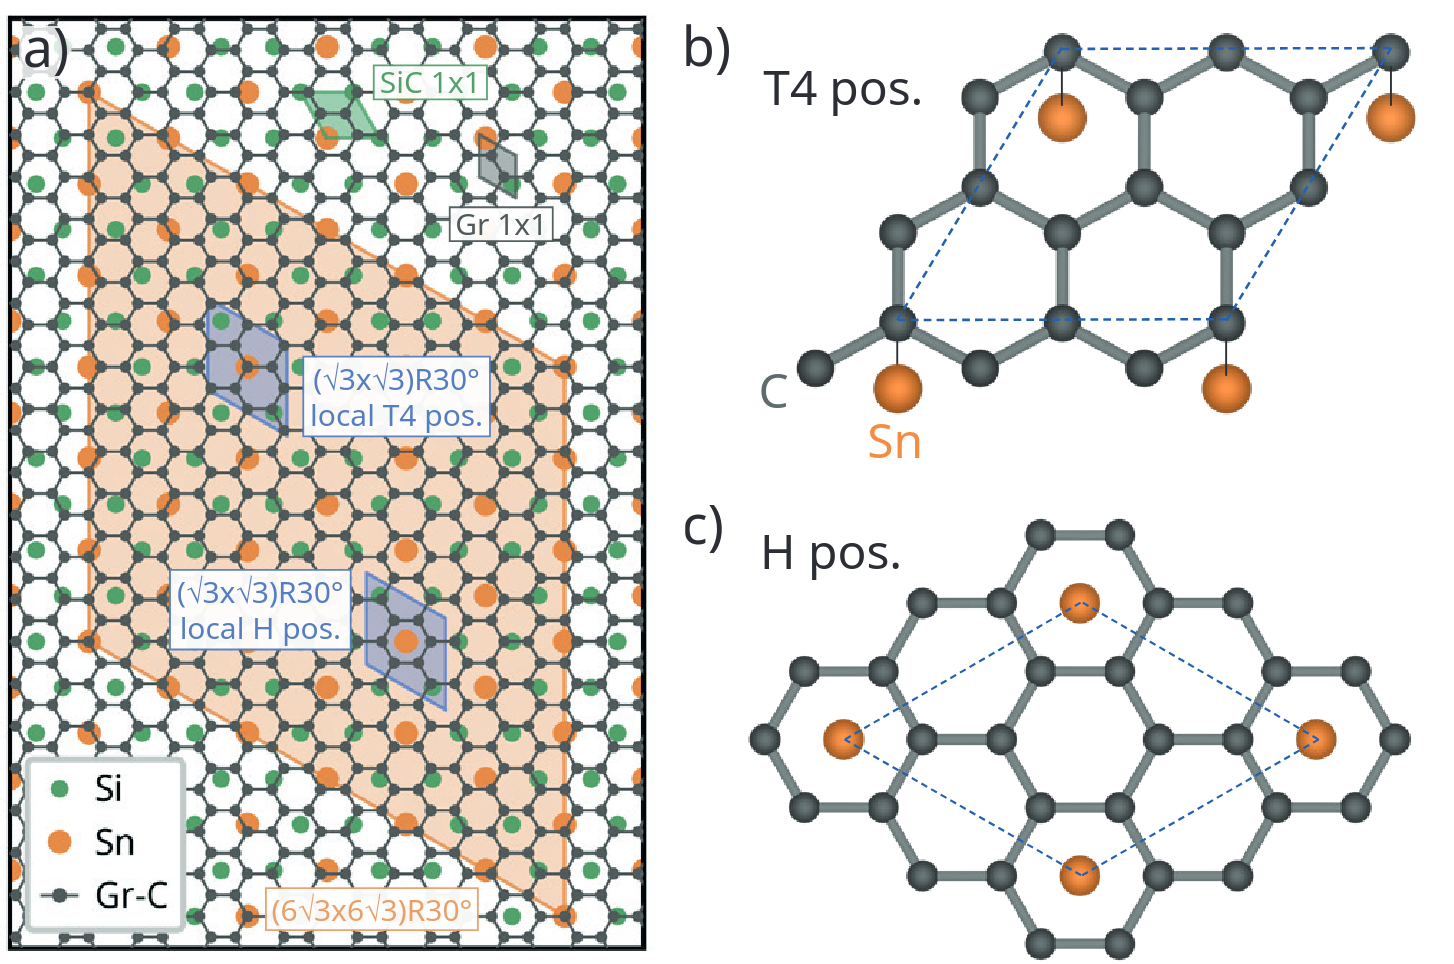
\includegraphics[width=\textwidth]{images/intercalated graphene experiment}
			\end{center}
		\end{column}
		\begin{column}{0.55\textwidth}
			\begin{center}
				\includegraphics[width=\linewidth]{"images/epitaxial graphene DFT different elements"}
			\end{center}
		\end{column}
	\end{columns}
\end{frame}


\begin{frame}
	\frametitle{Decorated Graphene Model\footnote[frame]{
			\citeauthor{wittQuantumGeometryLocal2025}\href{https://doi.org/10.48550/arXiv.2503.03700}{10.48550/arXiv.2503.03700} (\citeyear{wittQuantumGeometryLocal2025})
		}
	}
	
	\begin{columns}
		\begin{column}{0.45\textwidth}
			\begin{center}
				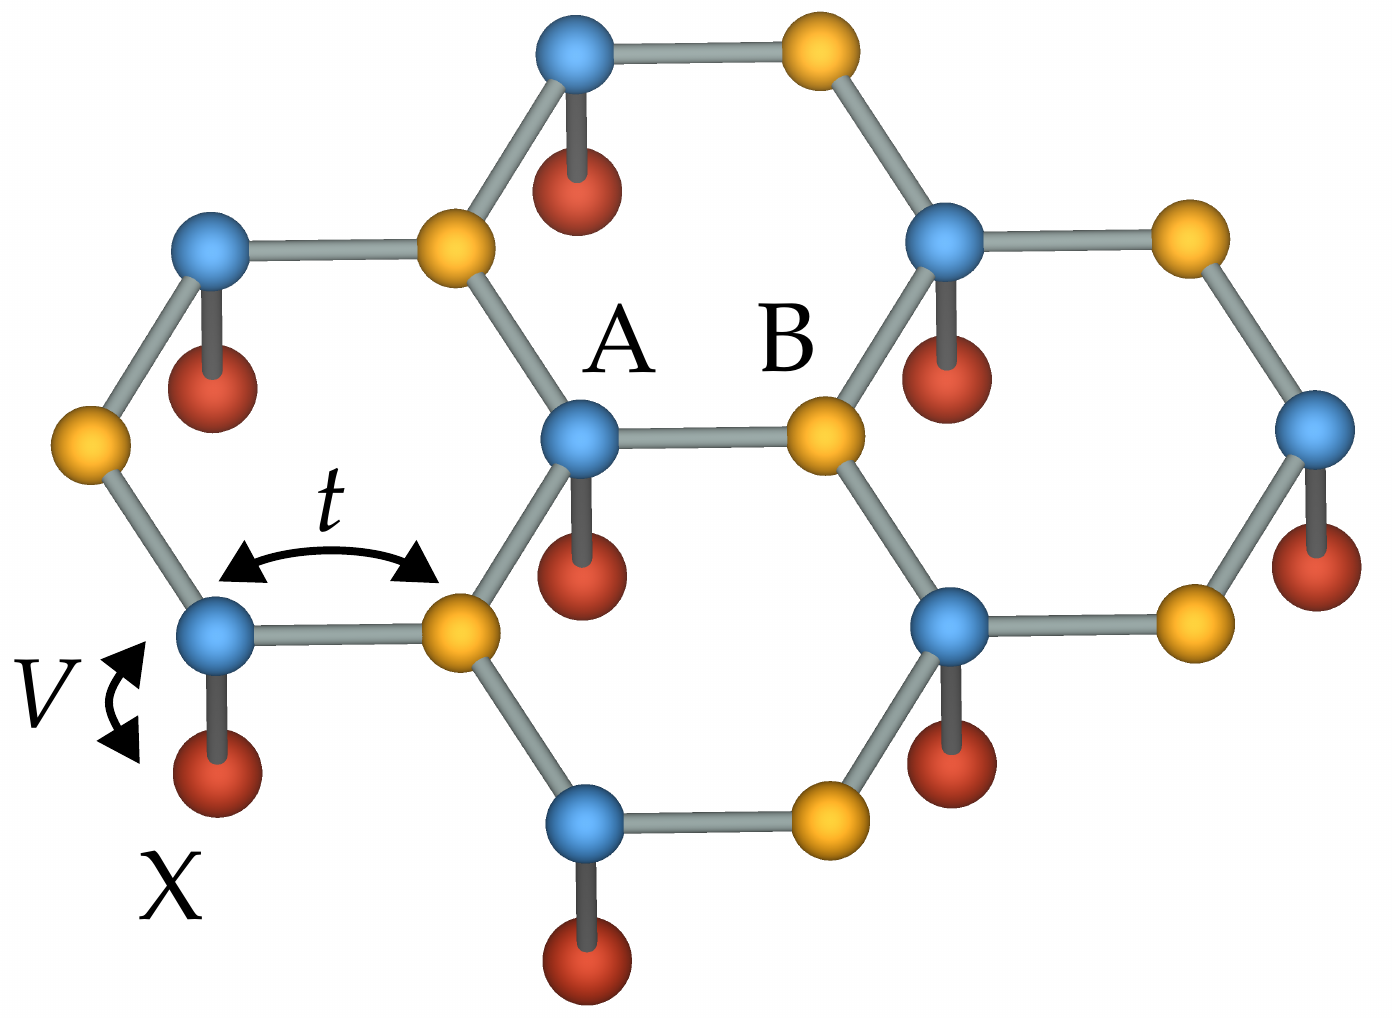
\includegraphics[width=0.7\textwidth]{images/decorated graphene lattice}
			\end{center}
			\begin{center}
				\includegraphics[width=\linewidth]{"images/decorated graphene band structure"}
			\end{center}
		\end{column}
		\begin{column}{0.55\textwidth}
			\begin{itemize}
				\item Captures essential elements: graphene lattice, flat band hybridized with graphene dirac cones
				\item Hamiltonian:
				\begin{align}
					H = &-t \sum_{\langle ij \rangle, \sigma}
					c_{i \sigma}^{(\mathrm{A}), \dagger} c_{j \sigma}^{(\mathrm{B})}
					+ V \sum_{i \sigma}
					d_{i \sigma}^{\dagger} c_{i \sigma}^{(\mathrm{A})} + \mathrm{h.c.} \nonumber \\
					&-\sum_{i, \alpha} U_{\alpha} c_{i \alpha \uparrow}^{\dagger} c_{i \alpha \downarrow}^{\dagger} c_{i \alpha \downarrow} c_{i \alpha \uparrow}
				\end{align}
			\end{itemize}
		\end{column}
	\end{columns}
\end{frame}


%\begin{frame}
%	\begin{columns}
%		\begin{column}{0.45\textwidth}
%			\begin{center}
%				\includegraphics[width=\linewidth]{"images/decorated graphene orbital weight"}
%			\end{center}
%		\end{column}
%		\begin{column}{0.55\textwidth}
%			\begin{itemize}
%				\item Shows 
%				\item Minimal quadratic Wannier spread:
%			\end{itemize}
%		\end{column}
%	\end{columns}
%\end{frame}

\begin{frame}
	\frametitle{Ginzburg-Landau Theory}
	
	Two ingredients:
	\begin{itemize}
		\item Order parameter:
		\begin{equation}
			\vert \Psi \vert =
			\begin{cases}
				0 & T \geq T_{\mathrm{C}} \\
				\vert \Psi (T) \vert > 0 & T < T_{\mathrm{C}}
			\end{cases} \;.
		\end{equation}
		\item Free energy: thermodynamic potential, minimized in thermodynamic equilibrium
		\item Ginzburg-Landau free energy (expansion of free energy in order parameter):
		\begin{equation}
			f_{\mathrm{GL}} [\Psi, \nabla \Psi] = \frac{\hbar^2}{2m^*} \vert \nabla \Psi \vert^2 + r \vert \Psi \vert^2 + \frac{u}{2} \vert \Psi \vert^4
		\end{equation}
	\end{itemize}
\end{frame}

\begin{frame}
	\begin{itemize}

		\item Writing \(\Psi = \vert \Psi \vert e^{\iu \phi}\):
		\begin{equation}
			f_{\mathrm{GL}}  = \frac{\hbar^2}{2m^*} \vert \Psi \vert^2 (\nabla \phi)^2 + \left[ \frac{\hbar^2}{2m^*} (\nabla \vert \Psi \vert)^2 + r \vert \Psi \vert^2 + \frac{u}{2} \vert \Psi \vert^4 \right]
		\end{equation}
		\item Correlation length:
		\begin{equation}
			\xi = \sqrt{\frac{\hbar^2}{2m^* \vert r \vert}} = \xi_0 \left(1 - \frac{T}{T_{\mathrm{C}}}\right)^{-\frac{1}{2}}
		\end{equation}
		with coherence length \(\xi_0 = \xi(T=0) = \sqrt{\frac{\hbar^2}{2 m^* \vert r \vert T_{\mathrm{C}}}}\)
		\item Coupling to electromagnetic field via vector potential \(\vb{A}\), i.e. \(f_{\mathrm{GL}} [\Psi, \vb{A}]\)
		\item Characteristic length scales for variations of \(\vb{A}\): London penetration depth \(\lambda_{\mathrm{L}}\)
	\end{itemize}
\end{frame}


%\begin{frame}
%	\frametitle{Why are these length scales important?}
%	
%	\begin{columns}
%		\begin{column}{0.4\textwidth}
%			\begin{center}
%				\includegraphics[width=\linewidth]{"images/critical current and magnetic fields"}
%			\end{center}
%		\end{column}
%		\begin{column}{0.6\textwidth}
%			\begin{itemize}
%				\item Critical fields and currents are deeply connected to the length scales
%				\item Characterize what is driving superconductivity: kinetic vs potential energy driven
%			\end{itemize}
%		\end{column}
%	\end{columns}
%\end{frame}

\begin{frame}
	\frametitle{Finite-Momentum Pairing Method}
	
	\begin{itemize}
		\item Stationary point of Ginzburg-Landau free energy:
		\begin{equation}
			\vert \Psi \vert = \vert \Psi_0 \vert \sqrt{1 - \xi^2 \vert \nabla \phi (\vb{r}) \vert^2}
		\end{equation}
		\item Breakdown of order parameter with phase fluctuations \(\to\) correlation length \(\xi\)
		\item Simple choice: \(\phi (\vb{r}) = \vb{q} \cdot \vb{r}\) \(\implies\) \(\xi \propto \frac{1}{q}\)
		\item Finite momentum \(\to\) current \(\vb{j}_{\vb{q}}\), can get 
		\begin{equation}
			\lambda_{\mathrm{L}} (T) \propto \sqrt{\frac{1}{\xi(T) j_{\mathrm{dp}} (T)}} \;,\; D_{\mathrm{S}} \propto \frac{1}{\lambda_{\mathrm{L}, 0}^2}
		\end{equation}
	\end{itemize}
\end{frame}

%\begin{frame}
	%Summary so far:
	
%	\begin{itemize}
%		\item Introduced length scales \(\lambda_{\mathrm{L}, 0}\) and coherence length \(\xi_0\)
%		\item Connect to critical fields and currents and can help characterize pairing
%		\item Can get information on length scales from the breakdown of the order parameter with phase fluctuations
%	\end{itemize}
%\end{frame}

\begin{frame}
	%\frametitle{FMP method in microscopic theories}
	
	BCS mean field theory
	\begin{itemize}
		\item \(H_{\mathrm{int}} \approx \sum_{i, \alpha} \left(\Delta_{i \alpha} c_{i \alpha \uparrow}^{\dagger} c_{i \alpha \downarrow}^{\dagger} + \Delta_{i \alpha}^{*} c_{i \alpha \downarrow} c_{i \alpha \uparrow}\right)\)
		\item Introduce FMP as \(\Delta_{i \alpha} = \Delta_{\alpha} e^{\iu \vb{q} \vb{r}_{i \alpha}}\)
		\item Mean-field Hamiltonian:
		\begin{align}
			H_{\mathrm{MF}} (\vb{q}) &= \sum_{\vb{k}} \Psi_{\vb{q}, \vb{k}}^{\dagger} 	\begin{pmatrix}
				H^{\uparrow}_{\vb{k}} - \mu & \Delta (\vb{q}) \\
				\Delta^{\dagger} (\vb{q}) & - \left(H^{\downarrow}_{\vb{q} - \vb{k}}\right)^* + \mu
			\end{pmatrix} \Psi_{\vb{q}, \vb{k}}
		\end{align}
		with \(\Psi_{\vb{q}, \vb{k}} = 
		\begin{pmatrix}
			c_{\vb{k} 1 \uparrow} & 
			c_{\vb{k} 2 \uparrow} &
			\ldots &
			c_{\vb{k} n_{\mathrm{orb}} \uparrow} &
			c_{\vb{q} -\vb{k} 1 \downarrow}^{\dagger} &
			c_{\vb{q} -\vb{k} 2 \downarrow}^{\dagger} &
			\ldots &
			c_{\vb{q} -\vb{k} n_{\mathrm{orb}} \downarrow}^{\dagger}
		\end{pmatrix}\)
	\end{itemize}
\end{frame}

%\begin{frame}
%	DMFT
%	\begin{itemize}
%		\item Nambu-Gor'kov Green's functions set up via:
%		\begin{align}
%			[\mathcal{G}_{\vb{q}} (\iu \omega_n, \vb{k})]^{-1} = \begin{pmatrix}
%				(\iu \omega_n + \mu) - h (\vb{k}) - \Sigma^{N} (\iu \omega_n) & -\Sigma^{\mathrm{AN}} (\iu \omega_n) \\
%				-\Sigma^{\mathrm{AN}} (\iu \omega_n) & (\iu \omega_n - \mu) + h (\vb{q} -\vb{k}) + (\Sigma^{N})^* (\iu \omega_n) \nonumber
%			\end{pmatrix}
%		\end{align}
%	\end{itemize}
%\end{frame}

\begin{frame}
	\frametitle{Superconductivity in Decorated Graphene}
	
	\begin{columns}
		\begin{column}{0.3\textwidth}
			\begin{center}
				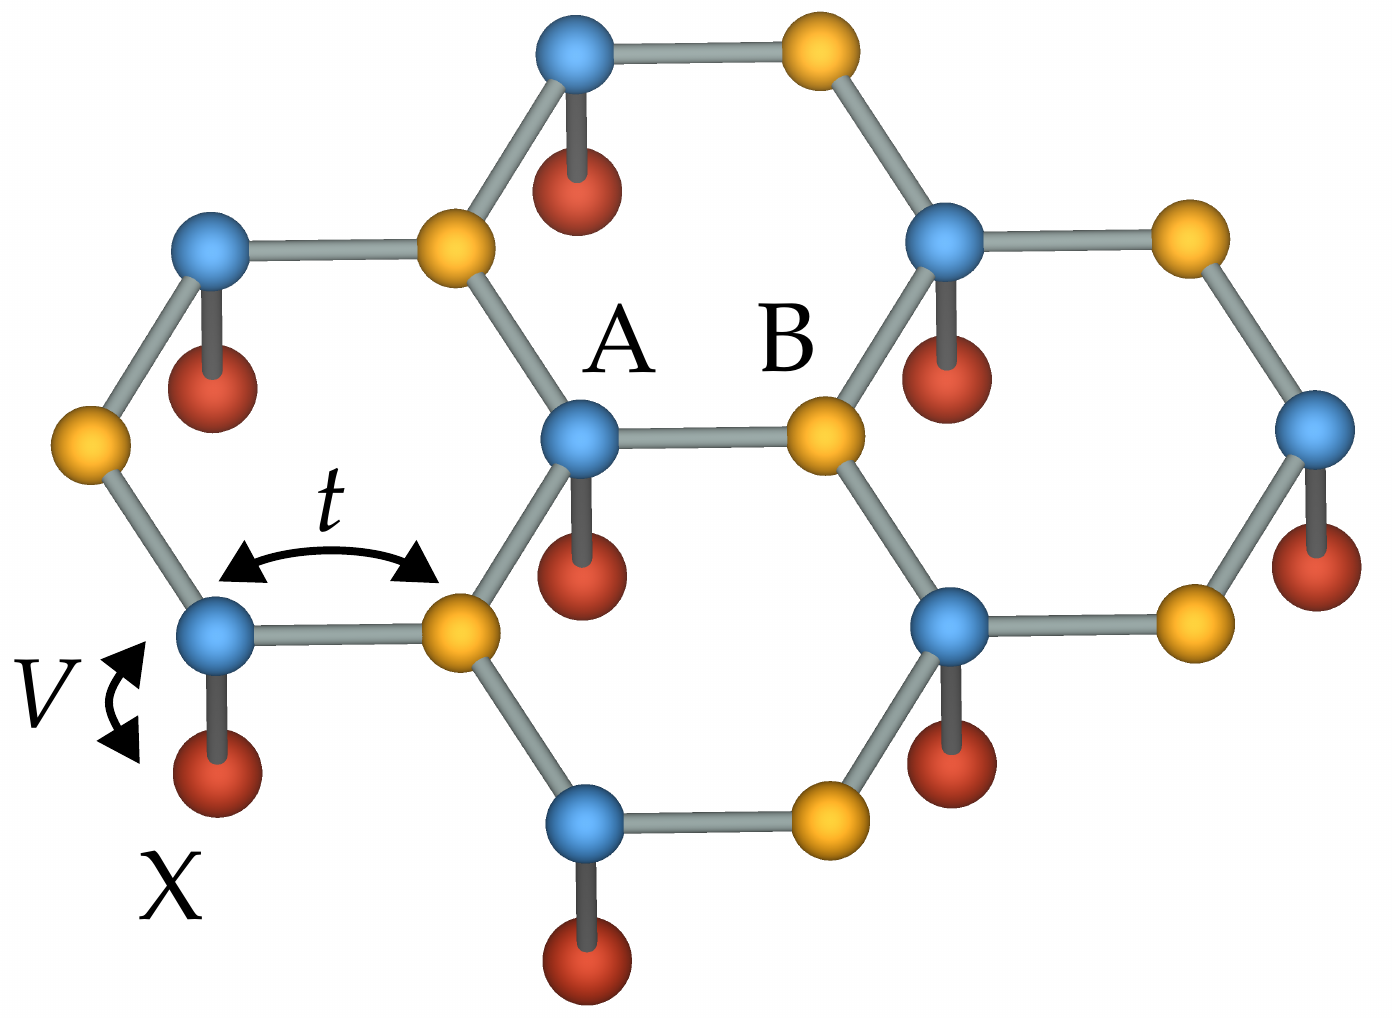
\includegraphics[width=\textwidth]{images/decorated graphene lattice}
			\end{center}

		\end{column}
		\begin{column}{0.35\textwidth}
			\begin{center}
				\includegraphics[width=\linewidth]{"images/decorated Graphene T_C"}
			\end{center}
		\end{column}
		\begin{column}{0.35\textwidth}
			\begin{center}
				\includegraphics[width=0.85\linewidth]{"images/decorated Graphene gaps vs V"}
			\end{center}
		\end{column}
	\end{columns}
	\begin{itemize}
		\item \(U = 0.1t\), results in range of \(T_{\mathrm{C}} = \qtyrange{150}{250}{\kelvin}\)
	\end{itemize}
\end{frame}


\begin{frame}
	\frametitle{FMP and Length Scales}
	
	\begin{itemize}
		\item Self-consistent calculation under finite \(\vb{q}\) (both for \(V = 1.5t\))
	\end{itemize}
	
	\begin{columns}
		\begin{column}{0.5\textwidth}
			\begin{center}
				\includegraphics[width=\linewidth]{"images/q breakdown of gap"}
			\end{center}
			\begin{itemize}
				\item Marked: points where \(\nicefrac{\Delta}{\Delta_0} = \nicefrac{1}{\sqrt{2}}\)
			\end{itemize}
		\end{column}
		\begin{column}{0.5\textwidth}
			\begin{center}
				\includegraphics[width=0.5\linewidth]{"images/sc current with q"}
			\end{center}
			\begin{itemize}
				\item Marked: maximum \(j_{\mathrm{dp}}\)
			\end{itemize}
		\end{column}
	\end{columns}
\end{frame}

\begin{frame}
	\begin{center}
		\includegraphics[width=0.7\linewidth]{"images/decorated Graphene zero temperature length scales"}
	\end{center}
\end{frame}

\begin{frame}
	\begin{columns}
		\begin{column}{0.55\textwidth}
			\begin{center}
				\includegraphics[width=\linewidth]{"images/decorated graphene results SF weight"}
			\end{center}

		\end{column}
		\begin{column}{0.45\textwidth}
			\begin{itemize}
				\item Superfluid weight \(D_{\mathrm{S}} \propto \frac{1}{\lambda_{\mathrm{L}, 0}^2}\)
				\item Quadratic Wannier spread \(\Omega_{\mathrm{I}} = \Tr \mathcal{M}_{i j}\)
				\item Conventional and geometric contribution calculated from linear response theory\footnote[frame]{\citeauthor{liangBandGeometryBerry2017}, \href{https://doi.org/10.1103/PhysRevB.95.024515}{10.1103/PhysRevB.95.024515} (\citejournal{liangBandGeometryBerry2017} \citeyear{liangBandGeometryBerry2017})}
			\end{itemize}
		\end{column}
	\end{columns}
\end{frame}

\begin{frame}
	\frametitle{Summary}
	
	\begin{itemize}
		\item Decorated graphene: model for graphene adatom heterostructures with flat band hybridized to Dirac cones
		\item Introduced finite-momentum pairing method to calculate superconducting length scales
		\item Showed length scales calculated in BCS mean field theory
	\end{itemize}
\end{frame}

\begin{frame}
	\frametitle{Outlook}
	
	\begin{itemize}
		\item Current project: benchmark FMP method in DMFT for one band Hubbard model
		\item Compare FMP method in BCS with other results in flat band systems (e.g. Lieb lattice\footnote[frame]{\citeauthor{penttilaFlatbandRatioQuantum2025}, \href{https://doi.org/10.1038/s42005-025-01964-y}{10.1038/s42005-025-01964-y} (\citejournal{penttilaFlatbandRatioQuantum2025} \citeyear{penttilaFlatbandRatioQuantum2025})} as a standard example), clear up the discrepancies
		\item Apply FMP method to (more realistic) extended decorated Graphene model
	\end{itemize}
	
	\begin{center}
		\includegraphics[width=0.55\linewidth]{"images/extended decorated graphene"}
	\end{center}
\end{frame}

\begin{frame}
	\frametitle{Results: FMP Method in DMFT (One-Band Hubbard)}
	
	\begin{columns}
		\begin{column}{0.45\textwidth}
			\begin{center}
				\includegraphics[width=\linewidth]{"images/OBH DMFT results"}
			\end{center}
		\end{column}
		\begin{column}{0.55\textwidth}
			\begin{itemize}
				\item Characterizes what is limiting superconductivity: pairing for low \(U\), phase coherence for high \(U\)
				\item \(T_{\mathrm{C}}\) in mean-field theory follows gap
			\end{itemize}	
		\end{column}
	\end{columns}
\end{frame}

\end{document}

